\section{Návrh aplikace}
V následující kapitole je popsána architektura systému, který umožňuje běh cloud native aplikací v k8s clusterech podle požadavků definovaných v předchozí kapitole \linebreak Definice požadavků na běh distribuované databáze. Architektura systému je zobrazena na obrázku \ref{fig:vk8s-architecture}. Systém se skládá ze tří menších celků. Prvním část se skládá z Kubernetes API a databáze Etcd. Uživatelé interagují s touto částí, s jejíž pomocí vytvářejí zdroje, které jsou dále distribuovány do jednotlivých clusterů. Druhá část systému se stará o distribuci uživatelských zdrojů do zvolených clusterů. Tato část se nazývá Controller. Třetí část je tvořena k8s clustery, které jsou umístěné v různých lokacích a zajišťují běh zvolených aplikací.\par
První část, která se skládá pouze z k8s API a Etcd databáze, je vstupní bod pro uživatele, kteří budou vytvářet své aplikace. Tento koncept je převzatý z k8s Master serveru, ovšem bez služeb Controller Manageru a Scheduleru. K8s API umožnuje vytvářet nové definice zdrojů a manipulaci s nimi. Konfigurace je uložena v databázi Etcd. Uživatelé mohou použít existující řešení pro správu k8s zdrojů jako je webové rozhraní k8s nebo nástroj kubectl pro správu k8s z příkazového řádku. Tyto nástroje umožňují také monitorování jednotlivých zdrojů. Na obrázku můžeme vidět, že Customer 1 vytvořil v přiděleném namespacu Deploymenty D1, D2, D3. Každý Deployment se skládá z N kontejnerů, které jsou označeny Pn. Zdroje, které se nachází v tomto centrálním API budou nazývány jako virtuální zdroje. Například virtuální Deployment D1 prozatím existuje pouze v centrálním API v podobě předpisu jak by měl být spuštěn a provozován. API také obsahuje mechanismy pro autentifikaci uživatelů na základě definovaných pravidel. Pro oddělení zdrojů jednotlivých uživatelů jsou použity namespacy. Uživatelé tak budou moci pracovat pouze se zdroji v přiděleném namespacu. Tento přístup zajistí bezpečný a izolovaný přístup více uživatelů do systému. Jak je zobrazeno na obrázku, Customer 1, má možnost spravovat pouze zdroje v zeleném namespacu a nikdy nemá možnost interagovat se zdroji Customera 2 v oranžovém namespacu a naopak.\par
Úlohou Controlleru je distribuovat zdroje z centrálního API serveru do jednotlivých clusterů v různých lokacích podle definovaných pravidel. Controller sleduje databázi zdrojů v centrálním API. Pokud uživatel vytvoří nový Deployment, Controller zjistí tuto skutečnost a podle labelů, které jsou přiřazené tomuto Deploymentu vloží konfiguraci Deploymentu do k8s clusterů v požadovaných lokacích. Jak můžeme vidět na obrázku, všechny tři Deploymenty uživatele Customer 1 jsou spuštěny ve všech třech dostupných lokacích. Tato strategie je nejjednodušší. Deploymenty zákazníka Customer 2 jsou spuštěny pouze ve dvou ze tří lokací, konkrétně v New Yorku a Praze. Zákazník Customer 2 například nemá pobočku v Londýně a proto nepotřebuje spouštět aplikaci v tomto regionu. Customer 2 má ovšem možnost v budoucnu spustit svou aplikaci v lokaci Londýn pokud to bude potřebovat. Uživatel tak přes centrální API přidá label, který popisuje lokaci v Londýně. Tuto změnu Controller zjistí a vloží definici do k8s clusteru v lokaci Londýn. Controller také podporuje spustit v lokaci Londýn pro uživatele Customer 2 pouze Deployment D1. Proto aby uživatelé mohli monitorovat své zdroje z centrálního API, Controller sleduje k8s clustery v jednotlivých lokacích a zpět do centrálního API vkládá informace o jednotlivých zdrojích. Uživatelé tak například vidí stav jednotlivých podů a další informace o Deploymentech.\par
V jednotlivých lokacích je spuštěn plnohodnotný k8s cluster. Tento cluster spouští aplikace podle konfigurace, kterou obdžel od Controlleru. Jednotlivé clustery jsou samostatné rozhodovací jednotky, které jsou na sobě nezávislé. Při výpadku spojení na centrální API, aplikace běžící v clusteru stále fungují a mohou tak obsluhovat uživatele. Po obnovení spojení jsou data o aplikacích nahrána zpět do centrálního API. 

\begin{figure}[H]
  \begin{centering}
    
	  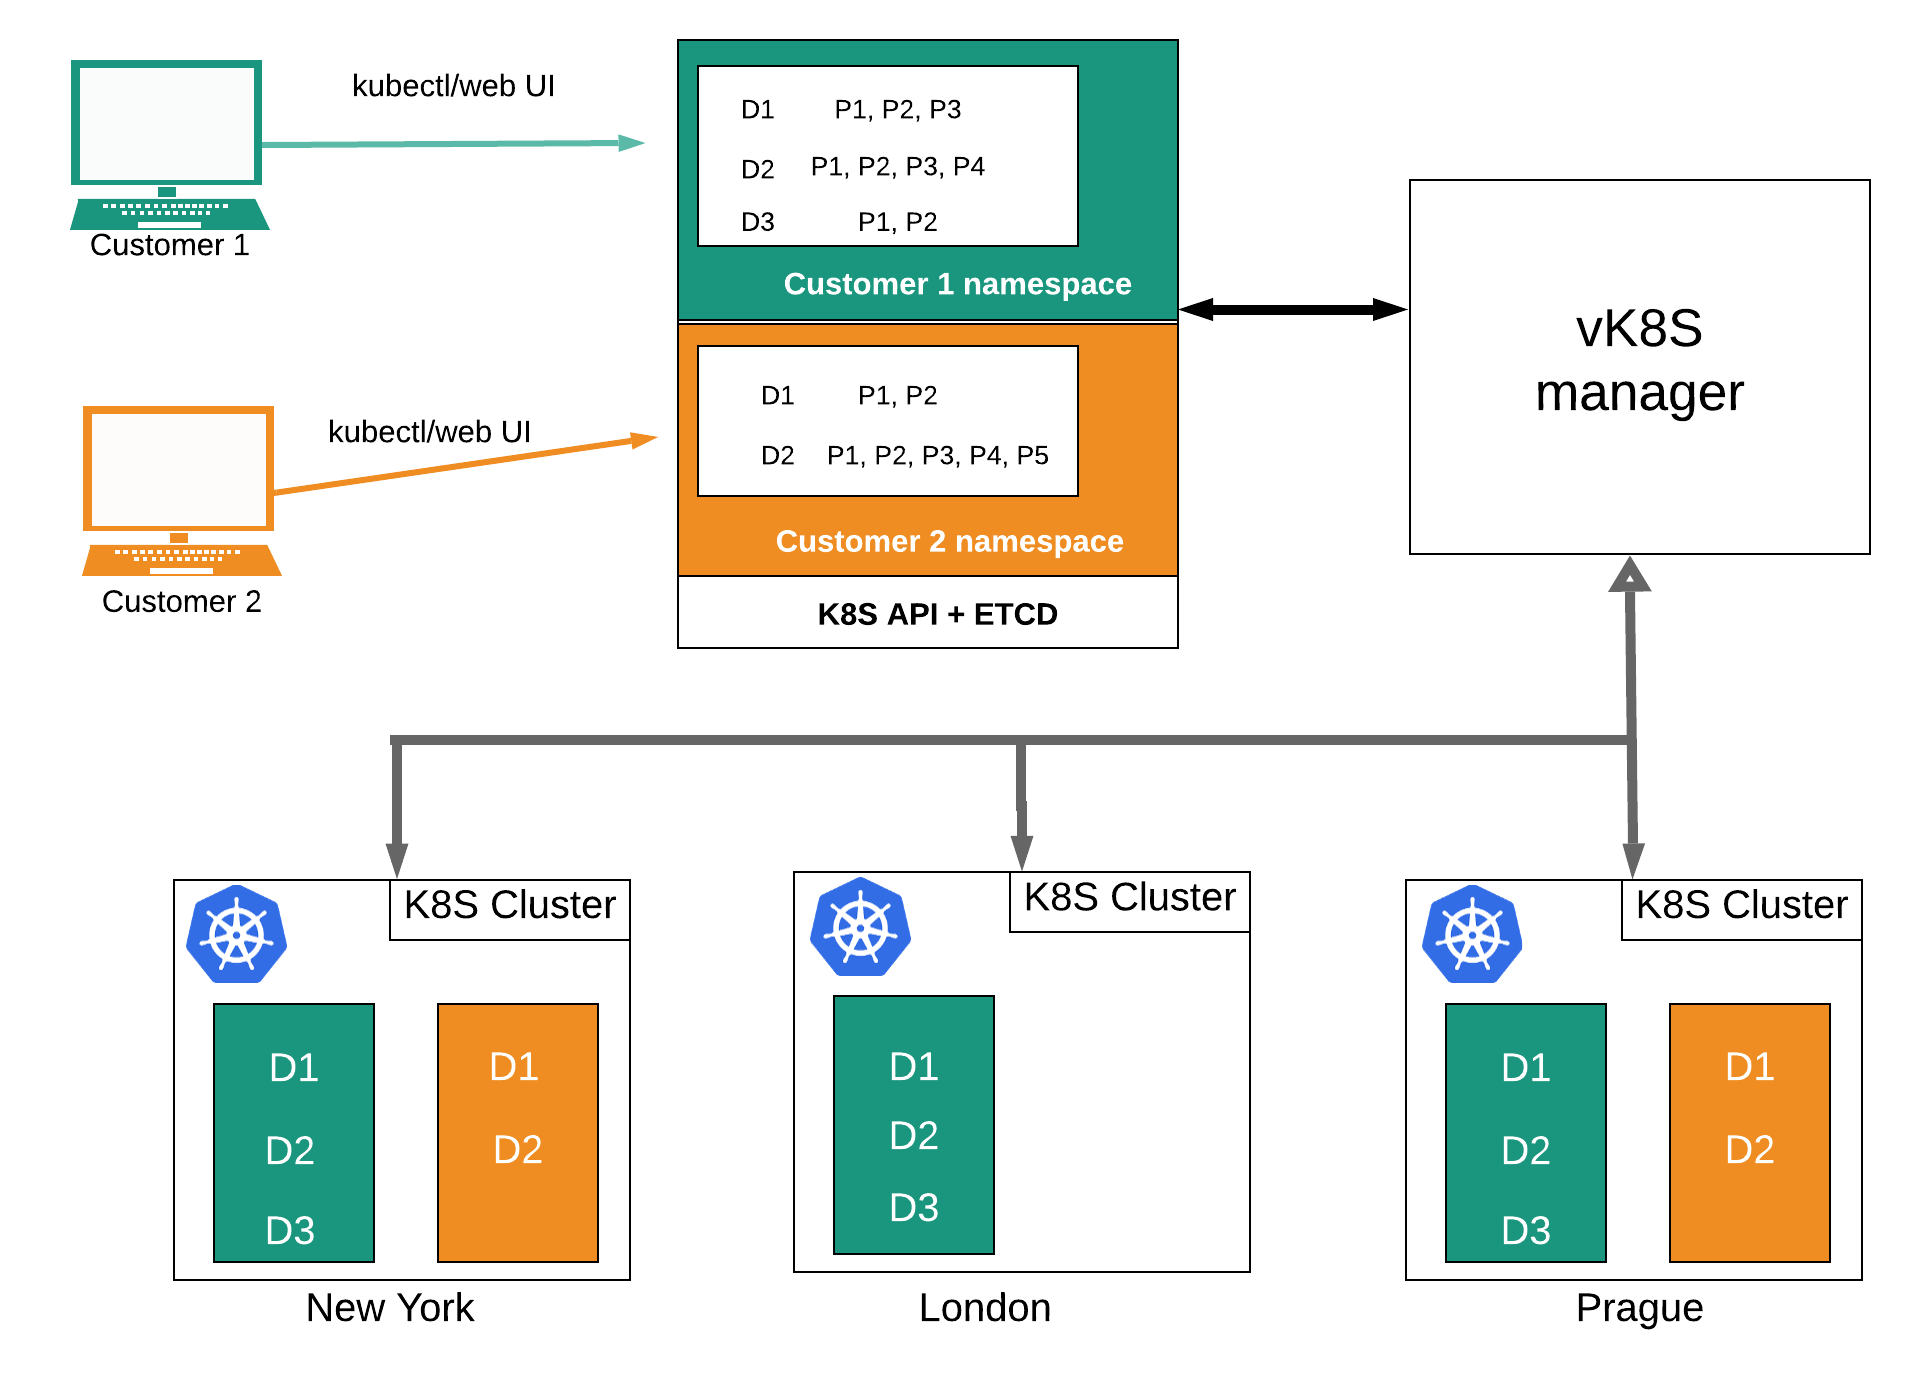
\includegraphics[width=0.8\textwidth]{images/vk8s-architektura.png}
    \par
	  \caption{Architektura navrhované aplikace\label{fig:vk8s-architecture}, zdroj: vlastní tvorba}
    \end{centering}
\end{figure}
